\section{Results}
To understand how value of contributions {\it flows} from editors to articles, and from articles to editors, we calibrated the control parameters $(\alpha^*,\beta^*)$ of the {\it bi-partite network random walker} on 12 Wikipedia categories (c.f. Table \ref{tab:statistics}) with 13 snapshots each (Figure \ref{fig:snapshots}). Figure \ref{fig:landscape} shows a typical optimization landscapes, which maximize the rank correlation $\rho_e$ between editors expertise $w_{e}$ obtained from the model and expertise obtained from state-of-the-art measures $\bar{w}_e$. The same is done for rank correlation $\rho_a$ between $w_a$ and $\bar{w}_a$. 

\begin{figure}[!t]
\centering
\includegraphics[width=0.9\columnwidth]{../Figures/contour_fem_combined.png}.
\caption{Typical landscape of maximum correlation as a function of $\alpha$ and $\beta$ for articles (upper panel) and editors (lower panel). The contour line shows the 95\textsuperscript{th} percentile of the rank correlation over the landscape. The category displayed here is {\it Feminist Writers}, for the largest snapshot ending February 2014.
\label{fig:landscape}
\end{figure}

The maximum achievable rank-correlation with ground-truth expertise metrics for editors \cite{geiger2013} and quality for articles \cite{wang2013tell} shows that the bi-partite model of influence accounts particularly well for both quality of articles ($0.58 < \rho_a < 0.91$) and expertise of editors ($0.46 < \rho_e < 0.75 $) at the last snapshot. Actually, the {\it bi-partite network random walker} model reproduces very well, and very early the ranking of editors and articles according to the ground-truth metrics (see Figure \ref{fig:rhotime}). In particular, articles quality is very well accounted for, while the level of correlation with the ground-truth of editors expertise exhibits a rather linear, or at least slightly concave increase.

%The question remains if the intersection of the solution spaces for $\rho_a$ and $\rho_e$ is nonempty. That is whether the we can find values of $\alpha$ and $\beta$ for which our editor ranking and article ranking are simultaneously optimized. We exploit two empirical facts from our data: the clear solution for article rankings that $alpha = 0$, and that for editor rankings the 95\textsuperscript{th} percentile maximizing boundary always includes values at $\alpha = 0$. Therefore, with $\alpha = 0$, we solve for $\beta$ in the editor ranking that maximizes $\rho_e$ - and thus $\rho_a$ simultaneously. 

For the latest snapshot (i.e., the state contributions in February 2014), we find that the best possible $\alpha^*$ is $0$ in all circumstances, and $\beta^*$ varies across categories. Table \ref{tab:maxbeta} shows the categories ordered by the optimal $\beta^*$ (and $\alpha^*=0$ for the sake of clarity), as well as the corresponding maximum rank correlations $\rho_e$ and $\rho_a$. Since there is no single optimal value for $(\alpha^*,\beta^*)$ , but rather a space of optimal values, we have searched for a value which maximizes both $\rho_e$ and $\rho_a$. $\alpha^* = 0$ means that editors expertise always benefits from contributions as a linear function of the number of articles edited (\textcolor{red}{and so on at higher orders}).  However, $\beta^*$ exhibits a continuum of values between $0$ ({\it Bicycle parts} and {\it US Military History}) and $1.52$ ({\it Sexual Acts"}). $\beta$ controls the non-linear influence of the number of editors on the quality of a given article. When $\beta \approx 0$, the quality of articles is increased as a linear function of the number of editors who have modified them. For $\beta \gg 0$, the marginal gain of having more editors for a given article decreases. So more editors touching does not improve an article that much.

$\beta$ is found generally stable over snapshots for categories, past the first 10\% of overall contributions. In fact $\beta$ switches signs only 3 times of the possible 144 measured changes. The times when $\beta < 0$ are in early history. Recall that the interpretation of $\beta < 0$ means that articles improve super-linearly with regards to number of editors - that is, very productive bursts. The stability of $(\alpha^*,\beta^*)$ confirm that the control parameters of the {\it bi-partite network random walker} describe a robust feature of the structure of value creation, at least in Wikipedia. This additional result is also a first step towards predictions of editors and articles, given the input made by editors.


\begin{table}
%\end{table}
\begin{tabular}{|llcccc|}
\hline
         &                     Category & $\rho_a$ & $\rho_e$ & $\alpha$ & $\beta$ \\
\hline
 1&                        Bicycle parts  &     0.90 &     0.46 &     0.00 &    0.00 \\
 2&Military history of the US  &     0.58 &     0.70 &     0.00 &    0.00 \\
  3&                Computability theory &     0.77 &     0.56 &     0.00 &    0.32 \\
   4&            American male novelists &     0.67 &     0.75 &     0.00 &    0.40 \\
    5&                        2013 films  &     0.72 &     0.55 &     0.00 &    0.48 \\
     6&                Economic theories  &     0.74 &     0.70 &     0.00 &    0.48 \\
     7&         American women novelists  &     0.63 &     0.75 &     0.00 &    0.64 \\
     8&                 Feminist writers  &     0.70 &     0.69 &     0.00 &    0.72 \\
     9&                             Yoga  &     0.64 &     0.57 &     0.00 &    1.12 \\
     10&      Nobel Peace Prize laureates  &     0.91 &     0.66 &     0.00 &    1.20 \\
      11&        Counterculture festivals  &     0.80 &     0.61 &     0.00 &    1.36 \\
        12&                   Sexual acts  &     0.63 &     0.66 &     0.00 &    1.52 \\
\hline
\end{tabular}
\caption{Categories ordered by increasing $\beta$ obtained from best rank-correlation $\rho_a$ and  $\rho_e$
 of the {\it bi-partite network random walker} with the ground truth. As shown on the upper panel of Figure \ref{fig:landscape}, highest rank-correlation is always obtained for $\alpha = 0$ suggesting that editors are experts in direct proportion to the number of articles they edit. The different values of $\beta$ show the effect of marginal editors on a article. As $\beta$ grows larger having more editors shows diminishing returns on article quality - "too many cooks spoil the broth".}
\label{tab:maxbeta}
\end{table}


%However, for categories with $\beta >0$ the quality of an article is also negatively influenced by the portfolio size of its editors. In other words, when $\beta$ is large, the more articles an editor edits, the lower his or her contributed value to one single article. $\beta$ also characterizes each category and the way quality is achieved through the cumulative contribution of information. For $\beta$ small, all editors have a fairly equal chance to contribute positively to any article, while for $\beta$ large, an editor can only contribute positively to a subset of articles (the larger $\beta$ the smaller the set). Typically, it is unlikely for a single person to have visited all {\it counterculture festivals}, performed all {\it sexual acts} or {\it Yoga} practices, while it is easier for anyone to gather relevant information on {\it bicycle parts} or the {\it US military history}. 





%\textcolor{red}{\bf Is there any reshuffling of ranking over time, or do they stay the same?}



\begin{figure}[!t]
\centering
<<<<<<< HEAD
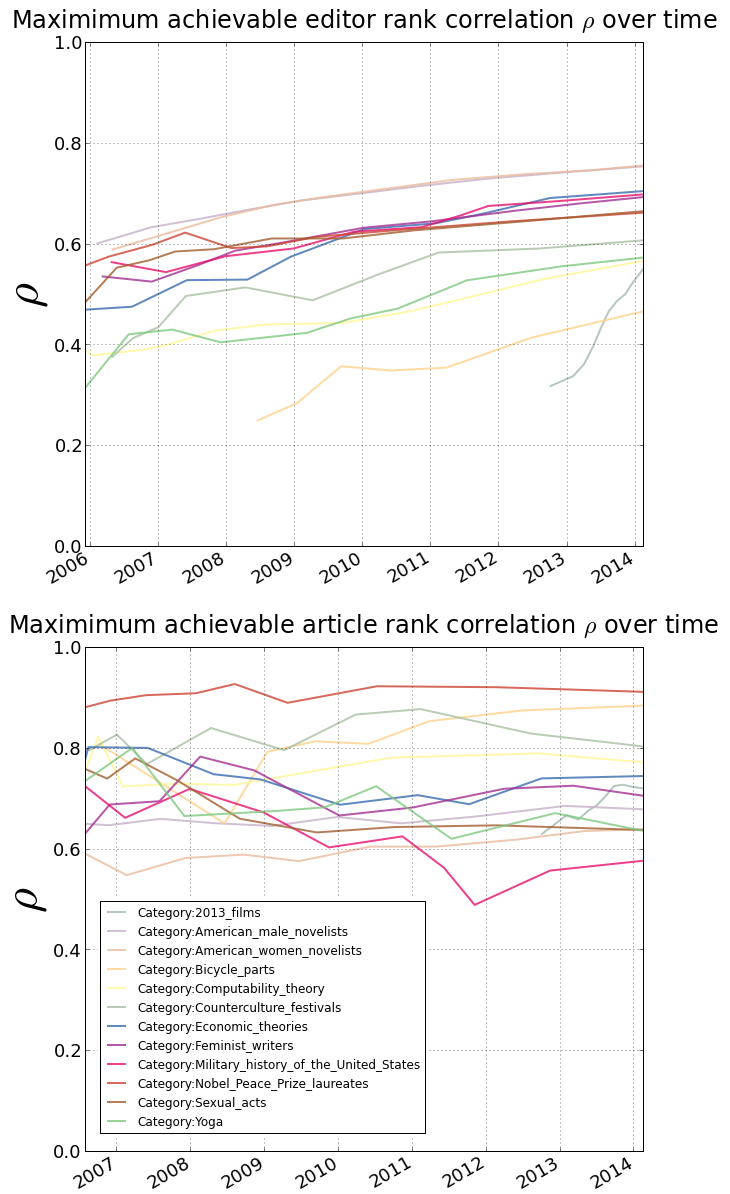
\includegraphics[width=0.9\columnwidth]{../Figures/rho_combined.png}.
\caption{Evolution of Spearman $\rho$ rank correlations between the ranking obtained from the calibrated model and the actual values for each category and for editors (upper panel)  and articles (lower panel). The correlations are generally quite high : $ 0.46 < \rho_e < 0.75$ with $\langle \rho_e\rangle = 0.64$ for editors and $0.57 < \rho_a < 0.91$ with $\langle \rho_a\rangle = 0.72$. $\rho_{a}$  is stable over time, which means that the quality of articles can be well captured early on by the model. However, $\rho_e$ exhibits a convex increase over time, suggesting that it takes time (i.e., lots of edits) to capture well the expertise of editors.}
\label{fig:rhotime}
=======
\includegraphics[width=0.9\columnwidth]{Figures/contour_fem_combined.png}.
\caption{Typical landscape of maximum correlation as a function of $\alpha$ and $\beta$ for editors (upper panel) and articles (lower panel). The contour line shows the 90th percentile of the rank correlation over the landscape. It typically displays a linear function between $\alpha$ and $\beta$. For articles, the relationship is typically of the type $\alpha = - b \beta + 1$ for $\beta >0$ or $\alpha = b \beta + 1$ for $\beta < 0$ with $b>0$ varying for each category. For editors, the relationship is $\alpha = 0$ for $\beta < ??$. {\it please add the corresponding figure for editors.  that would be great if you could make the labels ($\alpha$ and $\beta$) WAY bigger. You can also get remove the title. The cherry on the cake would be to have the color bar equal or smaller than the vertical dimension of the landscape, with keeping the landscape as a square rather than a rectangle.}}
\label{fig:landscape}
>>>>>>> 42d0243c97d914cb8b629e45dd5a716a2aafdd56
\end{figure}

	



